\section{Results}
\subsection*{\textbf{1b):} Developing your code and \textbf{1d):} A better statistical analysis}

The results of the simulations are included in the appendix as figures \ref{fig:1b_1} \ref{fig:1b_10}, \ref{fig:1b_100} and \ref{fig:1b_500}. The results were produced with the code in the repository\footnote{at commit \lstinline{b0ff612bc6666335b106af5e22a7a13a13c7cff7}}. Errors in the expectation value for the energy in the plots are computed with the blocking method\footnote{the blocking implementation is a copy of the code in Ref. \cite{ComphysGit}}. 
The exact answer for the minimum of the expecation value of the energy can be derived quote easily from \ref{eq:el_ni}. The minimum of the local energy has to be where the kinetic and potential energies cancel exactly. In the case of the 3d particle we see the following after imposing natural units. 

\begin{align}
\mathfrak{min}(E_L)  \implies \left(\frac{1}{2}\right)[4\alpha^2 (x^2 + y^2 + \beta^2 z^2) ] &= \frac{1}{2} (x^2 + y^2 + \beta z^2) \\
 2 \alpha ^2  &= \frac{1}{2} \\
 \alpha &= 0.5
\end{align}
With $\alpha$ at the minimum we then expect the following values for $\expect{E}$
\begin{equation}
\begin{split}
\text{1D: }E_L |_{\alpha = 0.5} &= \sum_i^N \alpha = N_ \alpha,\\
\text{2D: }E_L|_{\alpha = 0.5} &= \sum_i^N  2\alpha = 2N \alpha \\
\text{3D: }E_L|_{\alpha = 0.5} &= \sum_i^N  2\alpha + \alpha \beta  = 3N\alpha
\end{split}
\end{equation}
In general the energy in the non-interactive case at the variational minimum for our trial wavefunction can then be expressed as 
\begin{equation}
\mathfrak{min}(\expect{E[\alpha]}) = 0.5 \cdot N \cdot D  
\end{equation}
Where $N$ is the number of particles and $D$ is their dimension. From the figures referenced in the beginning of this section it is clear that both the numerical and analytic solutions converge to the correct solution.

\subsection*{\textbf{1e:} The repulsive interaction}

\begin{table}[]
    \centering
    \begin{tabular}{|c|c|c|c|c|c|}
    \hline
         $N$ & $\alpha$ & $\sigma^2$ & $\langle E_L \rangle$ & $\frac{\langle E_L \rangle}{N}$ & CPU-time [sek] \\
         \hline
         10 & 0.480013 & 1.73405e-06 & 21.643 & 2.1643 & 12.31 \\
         \hline
         50 & 0.480127 & 1.75833e-06 & 111.066 & 2.2213 & 1253.91\\
         \hline
         100 & 0.480279 & 1.75902e-06 & 228.682 & 2.2868 & 9854.01 \\
         \hline
    \end{tabular}
    \caption{VMC with Metropolis sampling. Calculations done in 3 dimensions with number of cycles $N_{MC} = 10^{6}$ for an elliptical trap, $\beta = 2.82843$ with interaction, $a = 0.0043$. Step length $t = 0.5$.}
    \label{tab:Re.int.}
\end{table}

Comment to be added to discussion: we see that the expectation value of the local energy increases by a small amount. This is consistent with what we see in Fig. 2 in (ref. to paper in Physics by J.L. DuBois). 


\subsection*{\textbf{1f:} Finding the best parameter}
Applying the gradient descent method to tune the variational parameter resulted in satisfying convergence to the optimal value for the variational parameter $\alpha$. The simulation results are included in figure \ref{fig:gd_nm_nia}\footnote{The simulations were produced with the file \lstinline{mainf_f.cpp} at commit \lstinline{2d03030ec5a711383d582dde23869483d122c6b6}}. After the convergence was shown to be satisfactory for the non-interactive case simulations were run for the hamiltonian with interaction \footnote{commit \lstinline{f285327a7d95349a874aafe16d8ecd5f48c5cef5}}. The result shows for the variational parameter as  $\alpha_{min} \approx 0.4988\ldots$. These findings are illustrated in figure \ref{fig:gd_nm_ia}. 


\begin{figure}
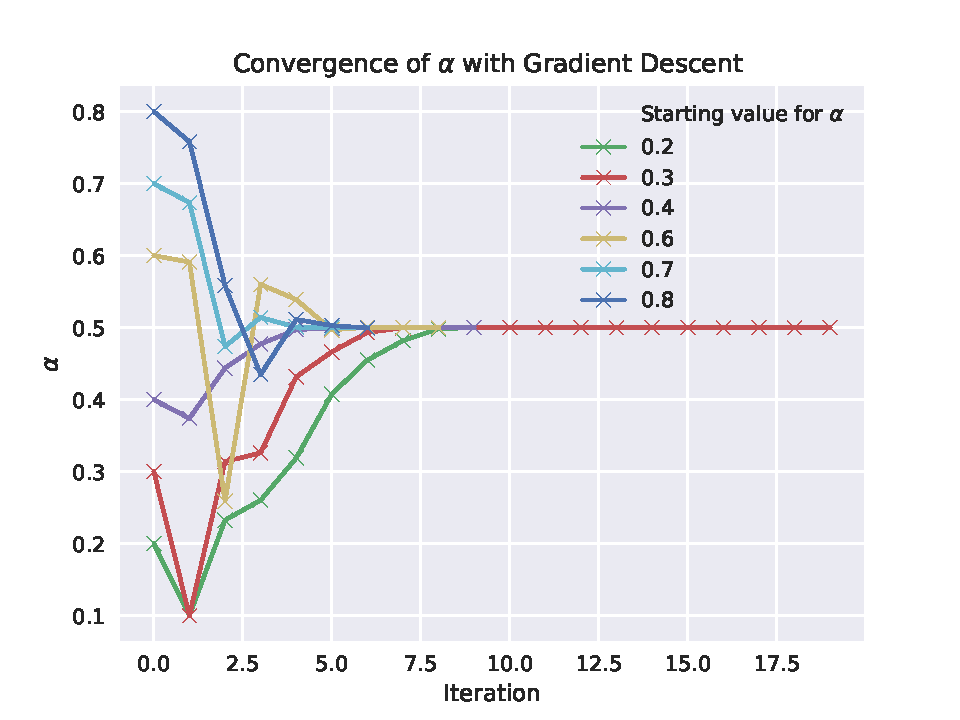
\includegraphics{figures/GD_NM_NIA.pdf}
\caption{Finding the optimal $\alpha$ with GD. This plot show the number of iterations it took to reach the minimum for the non-interactive spherical trap.}\label{fig:gd_nm_nia}
\end{figure} 

\begin{figure}
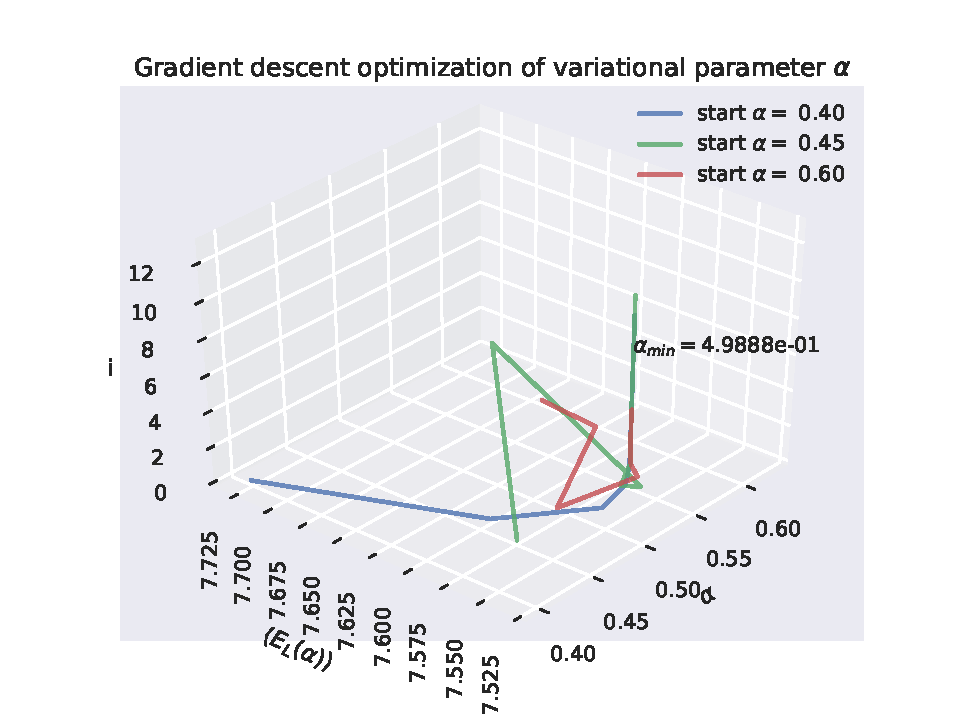
\includegraphics{figures/GD_NM_IA.pdf}
\caption{Finding the optimal $\alpha$ with GD. This plot shows the first central moment for the local energy on the y-axis, the variational parameter on the x axis and the GD iteration number on the z-axis for the interactive spherical trap. We observe that the GD algorithm finds a satisfyingly stable minimum with few iterations}\label{fig:gd_nm_ia}
\end{figure} 

\subsection*{\textbf{1g:} Onebody densities}

The onebody density was computed the counting of particles in areas around the origo. The origo was chosen as it is the natural focal point of particles in the harmonic oscillator as formulated in the project. The bins were equipartitioned by a set step length trivially determined as $\Delta L = L/n_{bins}$ where $L$ denotes the endpoint of the interval and $n_{bins}$ the total number of bins. The implementation of the algorithm can be found in \lstinline{vmc.cpp}. A simulation was run to compute the onebody densities for both the interactive and non-interacitve case for the respective minimas of the variational parameter $\alpha$. 

